\documentclass{beamer}

%%----Packages
\usepackage{fontspec}
% used to set font for the latex document.

\usepackage[CJKchecksingle]{xeCJK}
% using CJK to manage Chinese, need fontsec.
\setCJKmainfont[BoldFont={方正黑体简体}, ItalicFont={方正楷体简体}]{方正大标宋简体}
\setCJKsansfont{方正黑体简体}
\setCJKmonofont{方正中等线简体}

\usepackage{textcomp}    % provide symbols.

\usepackage{graphicx}
\graphicspath{{pic/}}
\usepackage{tikz}

\usetheme{PKULabMeeting}


\title{一个 PKULabMeeting 模版}
\author{小狼}
\institute{Peking University}    % provide the information of institute. 
\date{\today}
\logo{\includegraphics[height=0.6\textheight]{pku.png}}
\titlepagelogo{\includegraphics[width=0.3\textwidth]{pku.png}}
\titlepagebackground{\includegraphics[height=7cm]{gate.jpg}}
\department{School of Life Sciences}
\backgroundlogo{\includegraphics[height=4cm]{cloud.png}}


\begin{document}

%-*-coding:utf-8-*-

%%%%% This is the frames file of presentation.
%%%%% Author: Wolfson

\section*{Frontpage}

\begin{frame}
  \maketitle
\end{frame}


\section*{Contents}

\begin{frame}{Contents}
  \tableofcontents
\end{frame}


\section{Item}

\subsection{Itemize}
  
\begin{frame}{Itemize}
  \begin{itemize}
  \item<alert@1> blabla
  \item<alert@2> blabla
  \item<alert@3> blabla
  \end{itemize}
\end{frame}

\subsection{Enumerate}

\begin{frame}{Enumerate}
  \begin{enumerate}
  \item blabla
  \item blabla
  \item blabla
  \end{enumerate}
\end{frame}

\subsection{Enumerate}

\begin{frame}{Description}
  \begin{description}
  \item[who] blabla
  \item[what] blabla
  \item[how] blabla
  \end{description}
\end{frame}


\section{Block}

\begin{frame}{Block}
  \begin{block}{A Block Title}
    Some Words in the block
  \end{block}
\end{frame}

\section{Summary}

\begin{frame}{Summary}
  \begin{block}{A Title}
    Some Words
  \end{block}
\end{frame}


\section*{Acknowledgement}

\thanksframe{Thanks!}
 

 
\end{document}
